\documentclass[]{article}% insert '[draft]' option to show overfull boxes

%set up margins (gemetry package does more than just margins.)
\usepackage{geometry}
 \geometry{
	letterpaper,
	left=1in,
	top=1in,
	bottom=1in}

%This is the package that makes the nomenclature table.
\usepackage{nomencl}
\makenomenclature
%this will allow adjustment of nomenclature package in order to use multi cols and name the section myself without weird formatting.
\usepackage{xpatch}
\xpatchcmd{\thenomenclature}{%
 \section*{\nomname}% Look for `\section*... etc.
}{% Replace it by 'nothing'
}{\typeout{Success}}{\typeout{Failure}}

%% Useful packages
%Nominal Packages
\usepackage{amsmath} %package for math stuff

\usepackage{graphicx} %package for floats (figures)
\usepackage[colorlinks=true, allcolors=blue]{hyperref} %pacakge for hyperlinks (internal and external)
\usepackage{indentfirst} %package that indents first sentence of each paragraph.

%%Necessary Packages
%package used in nomenclature, not necessary if you change the format
\usepackage{multicol} %package allowing multiple columns

%Advanced Packages
\usepackage{xfrac} %package that allows slanted fractions rather than stacked ones, use \xfrac{}{} instead of \frac{}{}
\usepackage{siunitx} %package for SI units (see ftp://ftp.dante.de/tex-archive/macros/latex/exptl/siunitx/siunitx.pdf)
\usepackage{gensymb} %package for some convenient things in both math and text mode (see http://ctan.math.illinois.edu/macros/latex/contrib/was/gensymb.pdf)
\usepackage{wrapfig} %package allowing wrapping figures/tables in text (i.e., Di Vinci style)
\usepackage{caption} %package for advanced captioning
\usepackage{subfigmat}% packages automating layout for subfigures



%!!!!!---IGNORE EVERYTHING ABOVE THIS POINT IF YOU DON'T KNOW WHAT YOU'RE DOING.---!!!!!%
%How to learn what you're doing:
%This link is useful: https://www.sharelatex.com/learn/Main_Page
%As is this one: https://artofproblemsolving.com/wiki/index.php?title=LaTeX:Symbols
%And this one: google.com

%Change the Title Here:
\title{BYU FLOW Lab Semester Report Template}

%Put your name here:
\author{Student Name}
\date{\today} %Automatically puts in date when you compile.

%Document Actually begins here.
\begin{document}
% Add Title elements defined above. (autoformatted)
\maketitle

%Write the abstract here:
\begin{abstract}
Enter a short summary here. What topic did you investigate and why? What work did you perform? What were your main results and conclusion?
\end{abstract}

%Nomeclature is created here (automatically sorted alphabetically):
\section*{Nomenclature}
\smallskip
\begin{multicols}{2}
\printnomenclature
\end{multicols}
%Example of nomenclature delcaration (put these right next to where the symbol is used in the paper):
%\nomenclature{$mathematical symbol$}{Description}
%\nomenclature{$c$}{Speed of light in a vacuum inertial frame} %TODO: COMMENT THIS LINE OUT


\section{Introduction}
\label{sec:introduction}

Explain the context of the project, the methods you used, etc.  For this section and all following sections: If you refer to an equation, previous result or theory that is not regarded as common knowledge, then cite the source where you found it (unless you came up with it and this is the first publication in which it appears, of course). For example, you can cite the Nano 3 Lecture notes \cite{nano3} (whatever those are).

% You may consider adding a background section if appropriate
%\section{Background}
%\label{sec:background}

\section{Methods}
\label{sec:methods}

Explain the Methodolgy you used to produce your results.  Be specific. A reader should be able to exactly recreate your results based on what you write in this section.

\section{Results}
\label{sec:results}

What are your results? Show \textit{and} tell (use figures, etc.). What did you find? How does it compare to other physical models and/or experiements?

%Conlcusion = Discussion from IMRaD Model.
\section{Conclusion}
\label{sec:conclusion}

What conclusions do you draw from your results? What more needs to be investigated?

\begin{thebibliography}{9}
%this is a manual bibliography and is a pain...
\bibitem{nano3}
  K. Grove-Rasmussen og Jesper Nygård,
  \emph{Kvantefænomener i Nanosystemer}.
  Niels Bohr Institute \& Nano-Science Center, Københavns Universitet

\end{thebibliography}

%if you want to avoid pain and suffering in the form of writing out all your own bibliography stuff, you'll use the style of bibliography shown below, you just need a .bib file with all the bibliography info in it (use a reference manager for this)
% \bibliography{.bib_filename_relativepath}{}
% \bibliographystyle{aiaa} %pick a bibliography style according to where you are publishing.





\newpage
\appendix
\section{Some LaTeX tips from another template}
\label{sec:latex}
\subsection{How to Include Figures}

First you have to upload the image file (JPEG, PNG or PDF) from your computer to writeLaTeX using the upload link the project menu. Then use the includegraphics command to include it in your document. Use the figure environment and the caption command to add a number and a caption to your figure. See the code for Figure \ref{fig:frog} in this section for an example.

\begin{figure}[!ht]
\centering
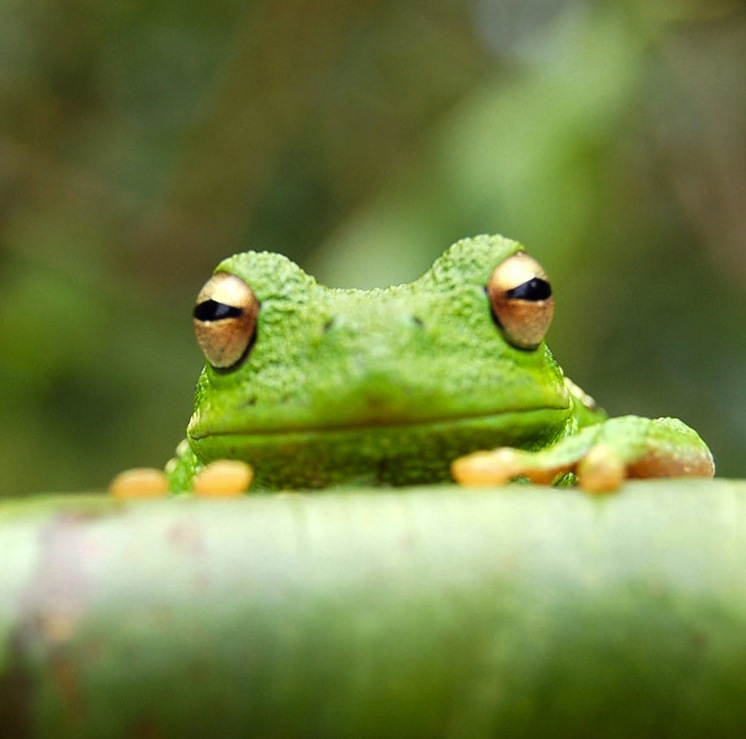
\includegraphics[width=0.3\textwidth]{frog.jpg}
\caption{This frog is in every \LaTeX template ever...}
\label{fig:frog}
\end{figure}

\subsection{How to Make Tables}

Use the table and tabular commands for basic tables --- see Table~\ref{tab:widgets}, for example.

\begin{table}[!ht]
\centering
\begin{tabular}{l|r}
Item & Quantity \\\hline
Widgets & 42 \\
Gadgets & 13
\end{tabular}
\caption{An example table.}
\label{tab:widgets}
\end{table}

\subsection{How to Write Mathematics}

\LaTeX{} is great at typesetting mathematics. Let $X_1, X_2, \ldots, X_n$ be a sequence of independent and identically distributed random variables with $\text{E}[X_i] = \mu$ and $\text{Var}[X_i] = \sigma^2 < \infty$, and let

\begin{equation}
S_n = \frac{X_1 + X_2 + \cdots + X_n}{n}
      = \frac{1}{n}\sum_{i}^{n} X_i
\label{eq:sn}
\end{equation}

denote their mean. Then as $n$ approaches infinity, the random variables $\sqrt{n}(S_n - \mu)$ converge in distribution to a normal $\mathcal{N}(0, \sigma^2)$.

The equation \ref{eq:sn} is very nice.

\subsection{How to Make Sections and Subsections}

Use section and subsection commands to organize your document. \LaTeX{} handles all the formatting and numbering automatically. Use ref and label commands for cross-references.

\subsection{How to Make Lists}

You can make lists with automatic numbering \dots

\begin{enumerate}
\item Like this,
\item and like this.
\end{enumerate}
\dots or bullet points \dots
\begin{itemize}
\item Like this,
\item and like this.
\end{itemize}
\dots or with words and descriptions \dots
\begin{description}
\item[Word] Definition
\item[Concept] Explanation
\item[Idea] Text
\end{description}

We hope you find write\LaTeX\ useful, and please let us know if you have any feedback using the help menu above.

\end{document}